\section{本システムの設計概要}
本研究では,行動別時間を可視化し,必要時間を簡単に算出させるため,ADLoggerシステムを提案する.
ADLoggerは行動時間を記録し,記録された時間を元にタスク別に必要時間を予測するiOSアプリケーションである.
クライアント側はタスク別時間記録モジュール,必要時間予測モジュール,カレンダー登録モジュール,アンケートモジュール,バッファ制御モジュール,表示制御モジュールから成る.
サーバ側ではデータベースへの書き込み及び読み込みを行う.

\begin{figure}[tb]
	\begin{center}
	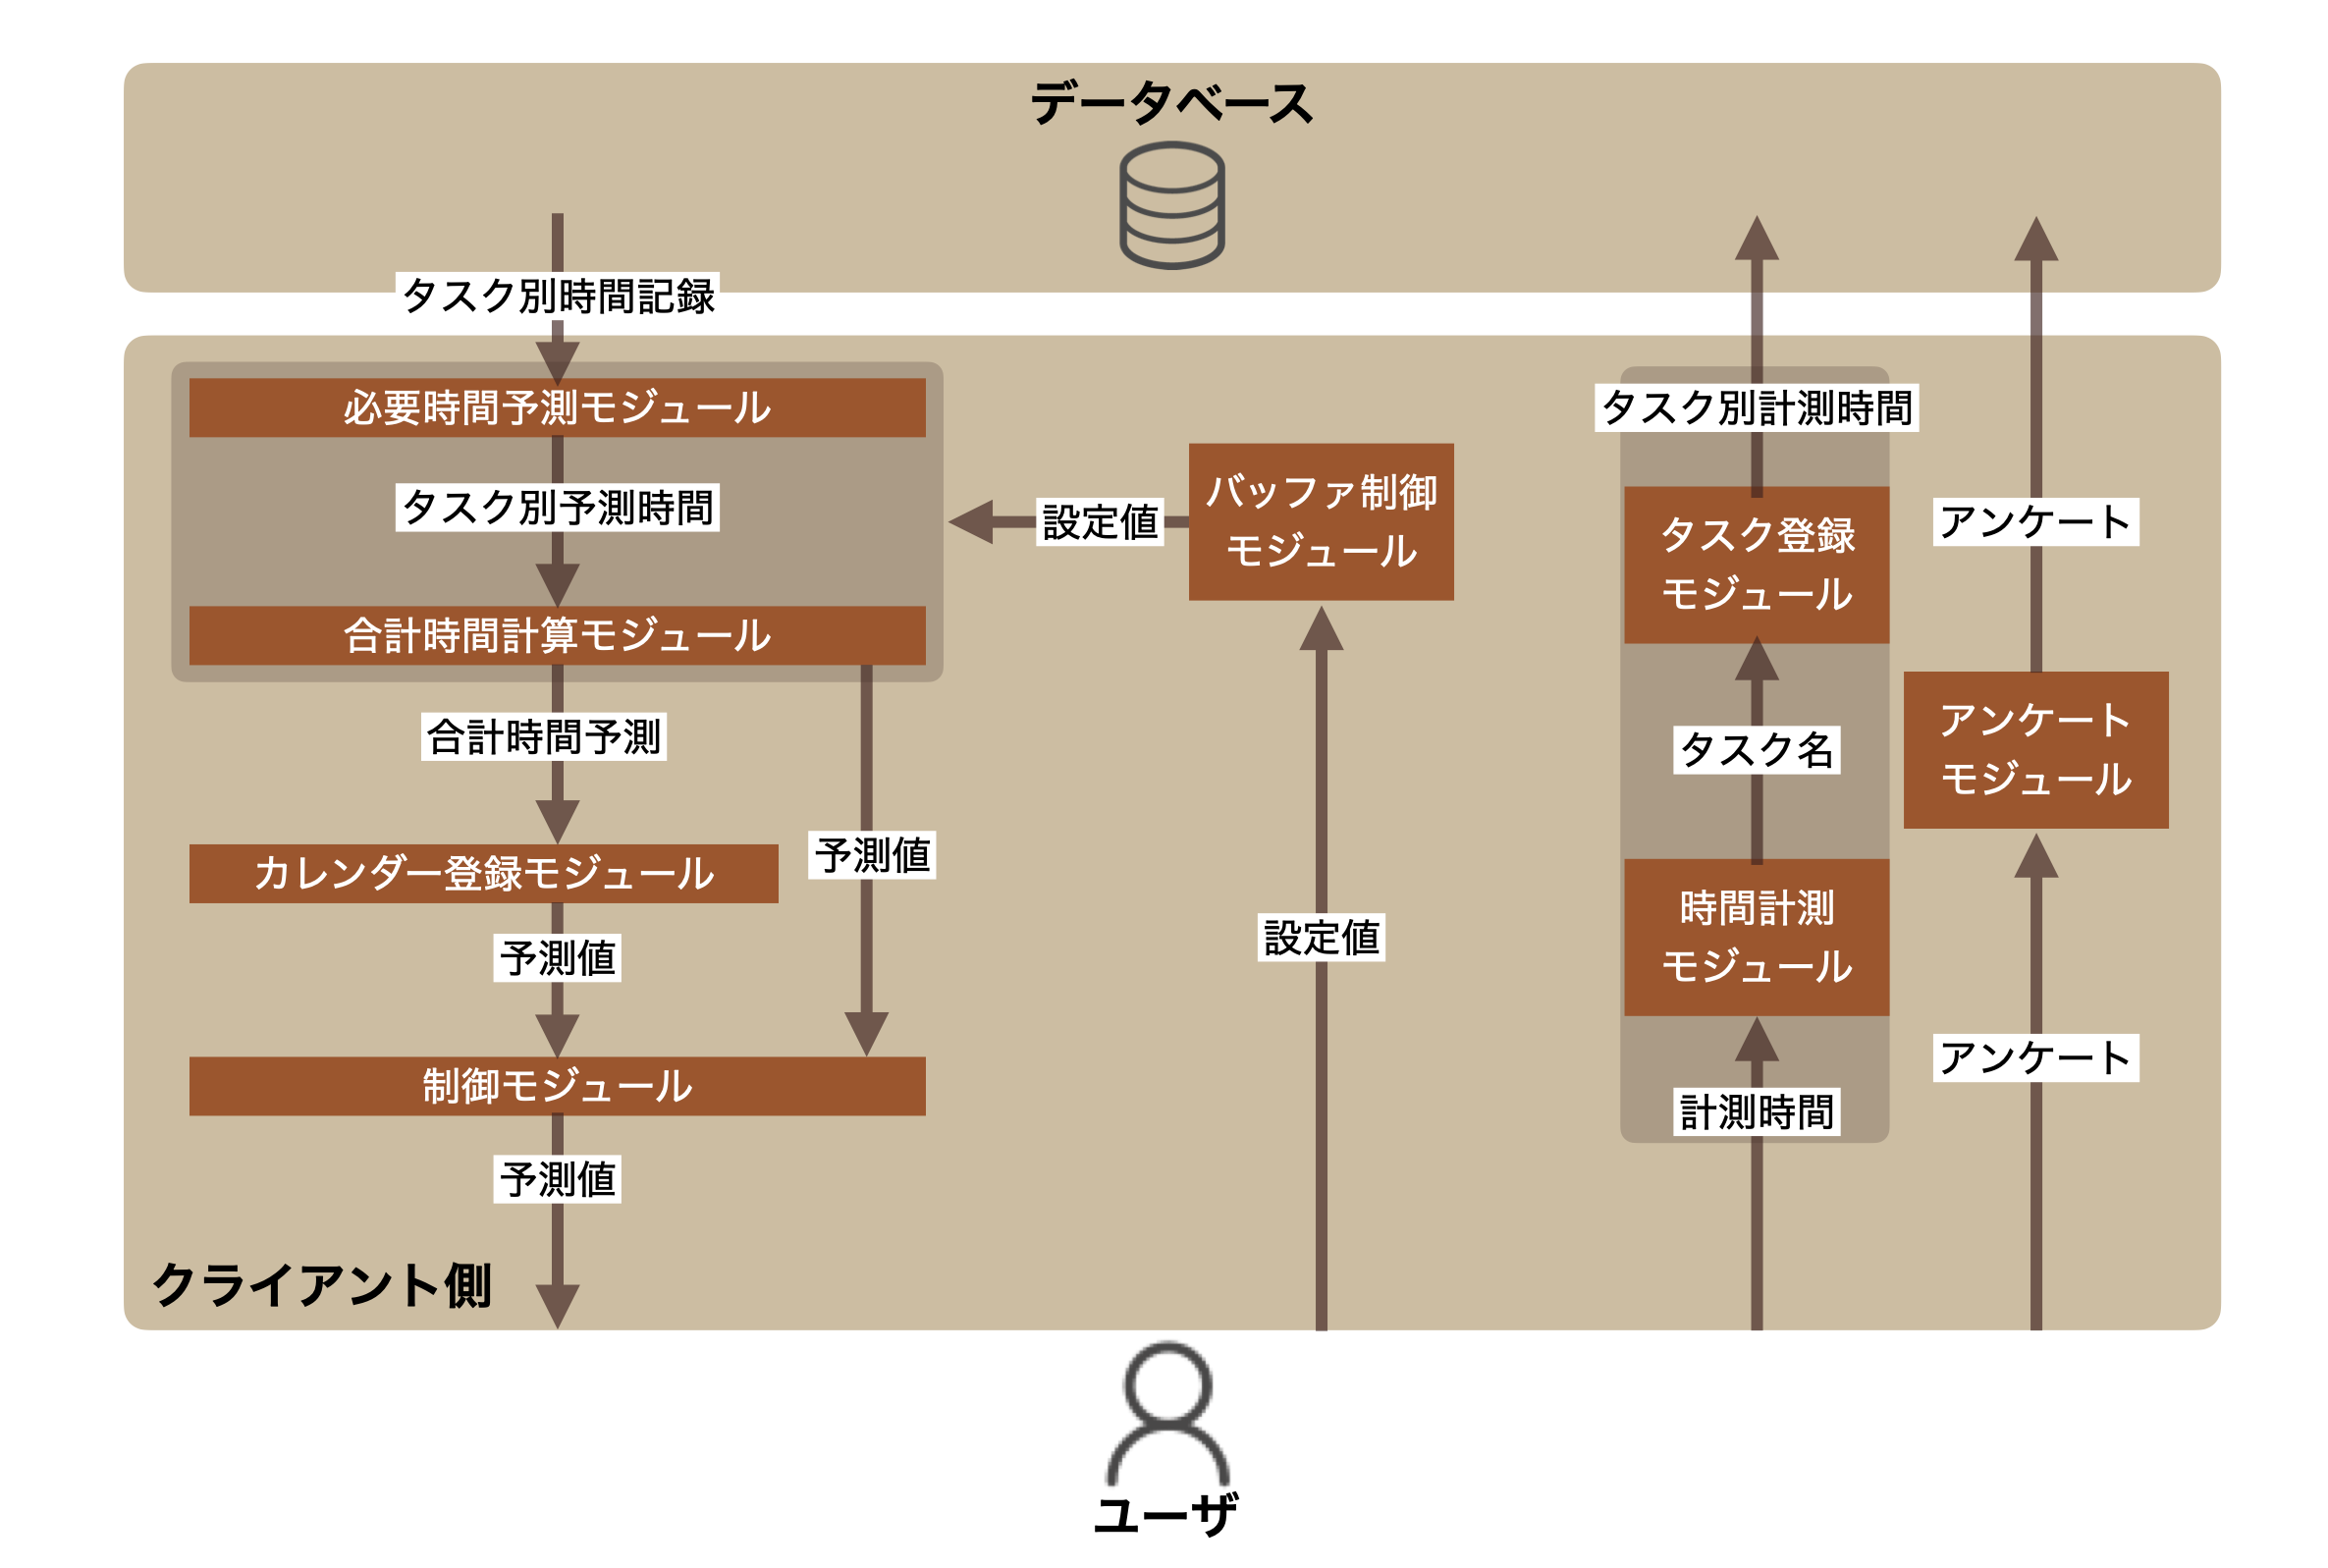
\includegraphics[width=16cm]{images/5/3.png}
	\end{center}
	\caption{システム構成図}
	\label{fig:system}
\end{figure}

\subsection{タスク別時間記録モジュール}
タスク別時間記録モジュールでは,ユーザが行動した時間をタスク別に記録を行う.
ユーザは本システムのストップウォッチを用いて時間を測定する.
時間の測定を終了するとタスク選択画面にて行った行動を選択する.
タスク選択画面には過去入力したタスク名がリスト形式で表示されており,新規タスクである場合は新規タスク名を登録する.

本モジュールはタスク名別に時間を記録し,サーバに送信する.
タスク別時間記録モジュールはユーザが行動したタスク及び時間を記録するモジュールである.
メイン画面のUIButton``TIMER"を押すと,ストップウォッチ画面に遷移する.(図~\ref{fig:stopwatch}参照)
UIButton``START"を押すとUIButtonが``STOP"に書き換えられた後,
上段に配置したUILabel``00:00:00"から “hh:mm:ss”の書式で書き換えられ経過時間が表示される.

\begin{figure}[ht]
\begin{center}
\begin{tabular}{c}

	\begin{minipage}[b]{0.5\linewidth}
	\begin{center}
		\fbox{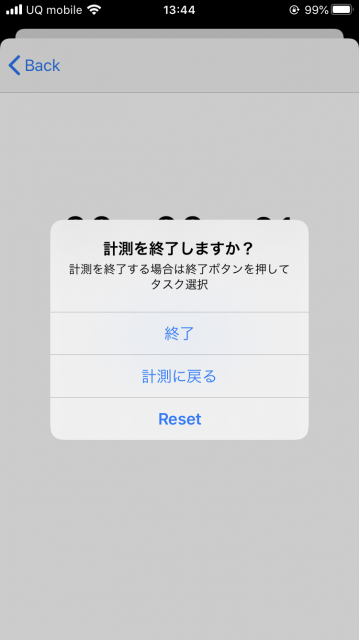
\includegraphics[width=5cm]{images/6/salert.png}}
		\caption{計測に関する選択}
		\label{fig:salert}
	\end{center}
  	\end{minipage}
	
	\begin{minipage}[b]{0.5\linewidth}
	\begin{center}
		\fbox{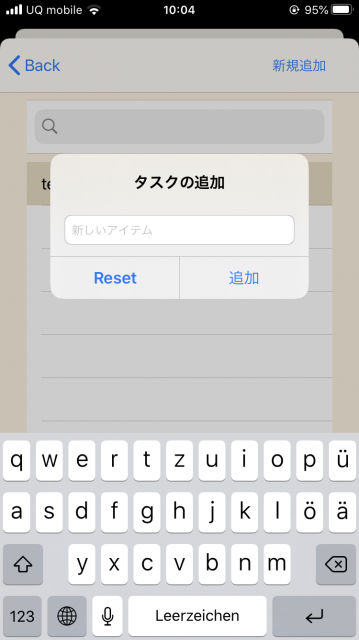
\includegraphics[width=5cm]{images/6/newtask.png}}
		\caption{新規追加}
		\label{fig:newtask}
	\end{center}
  	\end{minipage}
	
	\\
	
	\begin{minipage}[b]{0.5\linewidth}
	\begin{center}
		\fbox{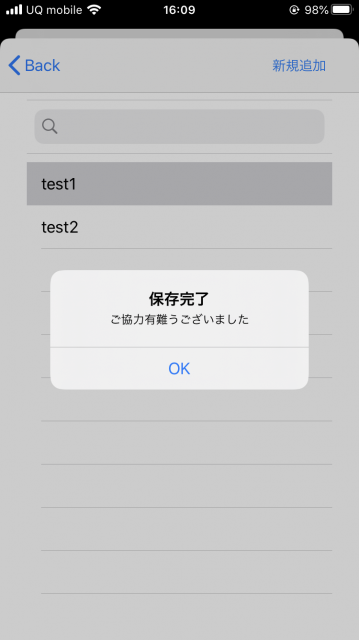
\includegraphics[width=5cm]{images/6/saved.png}}
		\caption{保存完了}
		\label{fig:saved}
	\end{center}
  	\end{minipage}
	
	\begin{minipage}[b]{0.5\linewidth}
	\begin{center}
		\fbox{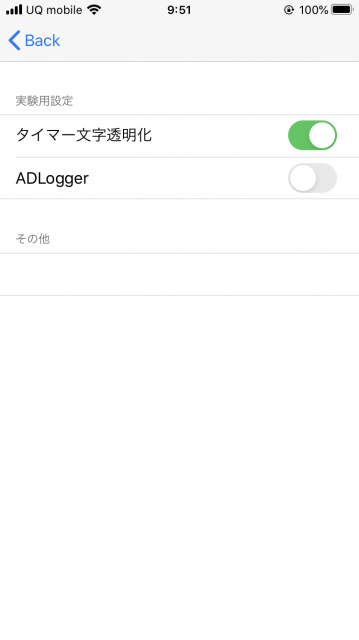
\includegraphics[width=5cm]{images/6/setting.png}}
		\caption{設定画面}
		\label{fig:setting}
	\end{center}
  	\end{minipage}

\end{tabular}
\end{center}
\end{figure}

\begin{figure}[ht]
\begin{center}
\begin{tabular}{c}

	\begin{minipage}[b]{0.5\linewidth}
	\begin{center}
		\fbox{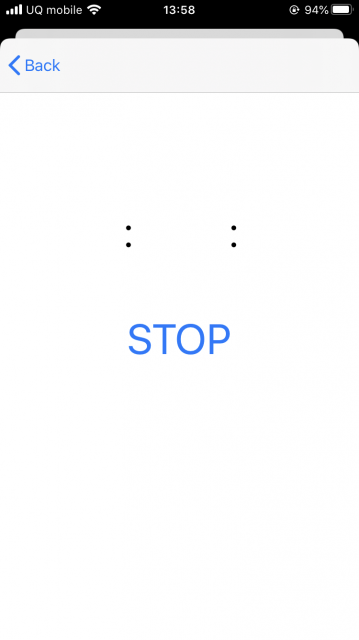
\includegraphics[width=5cm]{images/6/hidden.png}}
		\caption{ストップウォッチ画面の文字透明化}
		\label{fig:hidden}
	\end{center}
  	\end{minipage}

\end{tabular}
\end{center}
\end{figure}


再度UIButtonを押すとタスク別時間記録モジュールによって図~\ref{fig:salert}のようなUIAlertControllerが表示される.
このUIAlertControllerは,``終了"と``計測に戻る"と``Reset"の3つの選択肢を持っている.

``計測に戻る"を選択すると,UIButtonが``STOP"から``START"に書き換えられた後,上記の経過時間測定と同じ方法でカウントアップが再開される.
``Reset"を選択すると,上段の数字はカウントアップを終了しUILabelが``00:00:00"に書き換えられる事でリセット状態となる.
``終了"を選択すると現在のUILabelの値をInt型で変換した後,型で渡し,タスク選択画面へ遷移する.

タスク選択画面ではUITableViewで過去記録した事のあるタスク名が表示される.
各UITableViewCellに表示されているタスク名は,端末内のUserDefaultsにString型の配列として保存されている.
``新規追加"ボタンを押すと,UIAlertControllerが表示される(図~\ref{fig:newtask}).
このUIAlertControllerにはtextFieldが内蔵されており,新規タスクを記入しOKを押すとString型の配列に入力したtextFieldの値が新規タスクとして追加される.
UITableViewCellをタップすると記録した値がサーバーに送信され,保存が成功した事を示すUIAlertControllerが表示される(図~\ref{fig:saved}).
サーバに送られる値は表~\ref{tb:serverdata1}の通りである.尚,ユーザIDはログイン時に端末内のUserDefaultsで保存されたものを送信する.

\begin{table}[htb]
\begin{center}
  \caption{サーバに送信する値}
  \begin{tabular}{|l|l|}\hline
    サーバに送る値 & 型 \\ \hline
    ユーザID & PFUser型(サーバ指定のユーザ型) \\
    タスク名 & String型 \\
    記録時間(秒) & Int型 \\
    記録日時 & Date型 \\
	\hline
  \end{tabular}
  \label{tb:serverdata1}
\end{center}
\end{table}

\subsection{必要時間予測モジュール}
必要時間予測モジュールでは,ユーザの単一タスクないし選択された複数タスクの必要時間を予測する.
``ADLog"ボタンを押し算出画面に移動すると,タスク名毎の予測時間が自動計算されリスト形式で表示される.
リスト内のタスク名を選択すると,中央上段には選択タスクの合計必要時間が自動計算され結果が表示される.
また,同時に中央下段には合計必要時間で追加された合計バッファ時間が内訳として表示される.

メイン画面からUIButton``ADLog"を押すとADLog(必要時間予測)画面に推移される(図~\ref{fig:log}).
ADLog画面のUITableViewでは過去記録した事のあるタスク名とタスク毎の必要時間の予測が表示される.
まず,画面が読み込まれると同時にUserDefaultsに保存した値と一致するユーザIDをサーバで検索する.
該当するデータはタスク名(表~\ref{tb:tasktime_object}のtaskname)をkey,記録時間(表~\ref{tb:tasktime_object}のtasktime)をvalueとするDictionary型の配列を生成する.
valueは更にIntの配列としており,タスク名が重複された場合は記録時間をvalueの配列に追加する.
配列が生成し終わると平均時間$\bar{T}$を算出し,UITableViewCellの左側にタスク名,右側に平均時間$\bar{T}$を表示する.
UITableViewCellをタップすると中央一段目のUILabelを$T_{sum}$(数式(\ref{Ts}))の結果に書き換え,
中央二段目左のUILabelをタスクの$Tv$(数式(\ref{Tv}))の合計に,中央二段目右のUILabelを$Tf$に書き換える.
尚,$Tv$の$N$及び$Tf$は設定画面からのUserDefaultsによって決定される.
またUITableViewCellはaccessoryTypeにcheckmarkが指定されており,UITableViewCellがタップされると右側にチェックマークを表示しユーザが現在どのタスクを選択しているかを示す.

\subsection{カレンダー登録モジュール}
必要時間予測モジュールで算出された合計バッファ時間に関しては,タスク名,予定日時を入力し,
予定日時は開始時刻か終了時刻かの選択を行った上で``追加"ボタンを押すとappleのカレンダーに予定が登録される.

本モジュールはEventKitを用いて必要時間予測モジュールが算出した合計時間をAppleカレンダーに登録する.
カレンダー登録画面を開くと,ユーザが選択したタスクをもとに合計された$T_{sum}$(数式(\ref{Ts}))が受け渡されUILabelに表示される.
また,本モジュールにはカレンダーに登録したいタスク名を入力するUITextField,日時を決めるDatePickerが内蔵されたUIAlertController,DatePickerで選択したデータが開始時刻であるか終了時刻であるか決めるUISegmentedControlが存在する.
すべての項目を入力し,下部のUIButton``追加"を押すとAppleのカレンダーに入力の許可を確認した上で入力した値をカレンダーに渡し登録する事ができる.

\subsection{アンケートモジュール}
アンケートの質問に回答されたタスク名,タスク別所要時間,総合時間をサーバに送信する.
アンケートモジュールには複数のUITextFieldが搭載され,ユーザの入力した下記データをサーバに登録する.
\begin{table}[htb]
\begin{center}
  \caption{サーバに送信する値}
  \begin{tabular}{|l|l|} \hline
    サーバに送る値 & 型 \\ \hline
    ユーザID & PFUser型(サーバ指定のユーザ型) \\
    タスク名 & String型 \\
    タスク予測時間(秒) & Int型 \\
    総合予測時間(秒) & Int型 \\
    記録日時 & Date型 \\
	\hline
  \end{tabular}
  \label{tb:serverdata2}
\end{center}
\end{table}

\subsection{バッファ制御モジュール}
本システムではバッファ制御モジュールを通じてユーザは変動バッファ($Tv$)と固定バッファ($Tf$)を操作できる様にしている.
バッファ制御モジュールは設定画面にて操作が可能である.
変動バッファモードは``変更ボタン"を押すと``急ぎ"・``やや急ぎ"・``ややゆっくり"・``ゆっくり"の4つの選択肢が選べる.
選択肢によって数式(\ref{Tv})の$N$が変動し,必要時間予測モジュールに表示される色が下記の様に変化する(表~\ref{tb:buffer}).
\begin{table}[htb]
  \begin{center}
  \caption{バッファモードの選択分岐}
  \begin{tabular}{|c|c|c|} \hline
    モード & N & 表示色  \\ \hline \hline
    急ぎ & 0 & 赤  \\ \hline
    やや急ぎ & 1 & オレンジ  \\ \hline
    ややゆっくり & 2 & 緑  \\ \hline
    ゆっくり & 3 & 青  \\ \hline
  \end{tabular}
    \label{tb:buffer}
  \end{center}
\end{table}
固定バッファモードは設定画面に直接数字を入力し,``変更"ボタンを押すと入力した値を固定バッファとして計算式に追加する事が可能である.

設定画面はUITableViewで設計されており,2つのUITableViewCellがある.
UITableViewCellにはそれぞれUILabelが設置されており,``変動バッファモード"と``固定バッファ時間"と書かれている.

変動バッファモードのCellにはUIButton``変更"があり,UIButtonを押すとUIAlertControllerが現れる.
UIAlertControllerには``急ぎ"``やや急ぎ"``ややゆっくり"``ゆっくり"の4つの選択ができ,押すとそれぞれ0,1,2,3の値をUserDefaultsに登録できる.

固定バッファモードのCellには3つのUITextField及びUIButton``変更"が搭載されている.
3つのUITextFieldはそれぞれ時間,分,秒の入力を想定しており,入力しUIButton``変更"を押すと秒に変換しUserDefaultsに登録する.


\subsection{表示制御モジュール}
本モジュールは実験の関係上,最初は必要時間予測モジュールを使わず,経過時間を可能な限り閲覧できない環境にする為のものである.
表示制御モジュールは設定画面にて以下の制御が可能である(表~\ref{tb:hyoji}).
\begin{table}[htb]
\begin{center}
  \caption{表示制御モジュールの機能について}
  \begin{tabular}{|l|l|} \hline
   1 & 合計時間の算出画面へのロック機能 \\ \hline
   2 & ストップウォッチの透明化機能 \\ \hline
  \end{tabular}
  \label{tb:hyoji}
\end{center}
\end{table}
合計時間の算出画面へのロック機能は"ADLog"カラムを"OFF"にする事で"ADLog"ボタンから行動記録を見る事の制限をする事ができる.
ストップウォッチの透明化機能は"文字透明化"カラムを"ON"にする事でストップウォッチ作動時に時間経過のカウントアップが非表示となる.
初期設定は"ADLog"カラムを"OFF","文字透明化"カラムを" ON"としている.
いずれも"HELP"ボタンから閲覧できる"設定"ボタンの先にある設定画面からスイッチ形式で操作できる様にした.

設定画面はUITableViewで設計されており,2つのUITableViewCellによって成り立つ.
各UITableViewCellにはUISwitchが搭載されておりタップで操作が可能である.
初期設定は``文字透明化"が``ON",``ADLog"が``OFF"になっている.
``文字透明化"が``ON"だとストップウォッチ画面の経過時間を示すUILbelがhiddenとなり非表示となる(図~\ref{fig:hidden})
``ADLog"が``OFF"だとメイン画面のUIButton"ADLog"が機能せずUIButtonを押してもADLog画面に推移できなくなる.
ユーザがUISwitchを操作するとUserDefaultに保存され,状態が変化する.

\subsection{サーバ側設計}
サーバー側ではユーザ別に登録タスクとタスク時間記録をサーバ内にて管理する.
サーバ及びデータベースには,MBaaSであるBack4App~\cite{back4app}を利用する.
データベースにはユーザの認証情報を格納するUserクラスと, 行動時間記録を格納するtasktimeObject,アンケート 用のsurveyObject,survey2Objectが存在する.
Userクラスの例を表~\ref{tb:user_class},tasktimeObjectの例の例を表~\ref{tb:tasktime_object},surveyObjectの例の例を表~\ref{tb:survey_object},survey2Objectの例の例を表~\ref{tb:survey2_object}に示す.

\begin{table}[htb]
\begin{center}
  \caption{Userクラスの例}
  \begin{tabular}{|l|l|} \hline
  カラム名 & 値 \\ \hline
    objectId & ``2rg6ZJp7GQ" \\
    username & ``testuser" \\
    password & ``testpassword" \\
    ACL & ``2rg6ZJp7GQ" \\
   createdAt & 2020-7-6T07:24:08.810Z  \\
   updatedAt & 2020-7-6T07:24:08.810Z \\ \hline
  \end{tabular}
  \label{tb:user_class}
\end{center}
\end{table}

\begin{figure}[htb]
\begin{center}
\begin{tabular}{c}

\begin{minipage}[htb]{\linewidth}
\begin{center}
  \begin{tabular}{|l|l|} \hline
    カラム名 & 値 \\ \hline
    objectId & ``sRPnWYv0t6" \\
    username & ``testuser" \\
    taskname & ``test1" \\
    tasktiime & 561 \\ 
    createdAt & 2020-7-6T07:24:08.810Z  \\
    updatedAt & 2020-7-6T07:24:08.810Z \\ \hline
  \end{tabular}
   \caption{tasktimeObjectの例}
  \label{tb:tasktime_object}
\end{center}
\end{minipage}

\\

\begin{minipage}[htb]{0.5\linewidth}
\begin{center}
  \caption{surveyObjectの例}
  \begin{tabular}{|l|l|} \hline
    カラム名 & 値 \\ \hline
    objectId & ``9ooWCZj6mp" \\
    username & ``testuser" \\
    taskname & ``test1" \\
    tasktime & 561 \\ 
    createdAt & 2020-7-6T07:24:08.810Z  \\
    updatedAt & 2020-7-6T07:24:08.810Z \\ \hline
  \end{tabular}
  \label{tb:survey_object}
\end{center}
\end{minipage}

\begin{minipage}[htb]{0.5\linewidth}
\begin{center}
  \caption{survey2Objectの例}
  \begin{tabular}{|l|l|} \hline
    カラム名 & 値 \\ \hline
    objectId & ``bPs2GkrlkG" \\
    username & ``testuser" \\
    totaltime & 1320 \\ 
    createdAt & 2020-7-6T07:24:08.810Z  \\
    updatedAt & 2020-7-6T07:24:08.810Z \\ \hline
  \end{tabular}
  \label{tb:survey2_object}
\end{center}
\end{minipage}
\end{tabular}
\end{center}
\end{figure}